
\documentclass[10pt]{article}

\usepackage[a4paper,margin=0.65in]{geometry}
\usepackage{amsmath,amssymb}
\usepackage{graphicx}
\usepackage{booktabs}
\usepackage{array}
\usepackage{float}
\usepackage{hyperref}
\usepackage{enumitem}
\usepackage{xcolor}
\usepackage{tikz}
\usetikzlibrary{positioning,arrows.meta,shapes.geometric,fit,calc}

\setlist{nosep,leftmargin=*}
\renewcommand{\arraystretch}{1.2}
\setlength{\parindent}{0pt}
\setlength{\parskip}{2pt}

\tikzset{
layer/.style={
draw,
rounded corners,
minimum width=1.7cm,
minimum height=0.65cm,
align=center,
fill=blue!10,
font=\scriptsize
},
smalllayer/.style={
draw,
rounded corners,
minimum width=1.35cm,
minimum height=0.58cm,
align=center,
fill=green!10,
font=\scriptsize
},
arrow/.style={
-{Latex[length=2mm]},
thin
}
}

\begin{document}

%%%%%%%%%%%%%%%%%%%%%%%%%%%%%%%%%%%%%%%%%%%%%%%%%%%%%%%%%%%%
% TITLE
%%%%%%%%%%%%%%%%%%%%%%%%%%%%%%%%%%%%%%%%%%%%%%%%%%%%%%%%%%%%

\begin{center}

{\large\textbf{Shiv Nadar University Chennai}}

\vspace{2mm}

{\normalsize\textbf{CS3807 -- Deep Learning Laboratory}}

\vspace{2mm}

{\large\textbf{Experiment 6}}

\vspace{1mm}

{\normalsize\textbf{End-to-End Study of RNN, LSTM and GRU for}}

{\normalsize\textbf{Sequence Learning and Video Understanding}}

\end{center}

\vspace{3mm}

\begin{tabular}{|p{3.4cm}|p{9.0cm}|p{1.4cm}|}
\hline
Degree \& Branch &
B.Tech Artificial Intelligence \& Data Science &
Semester V\\
\hline
Subject Code \& Name &
CS3807 -- Deep Learning Laboratory &
AY: 2026--27\\
\hline
\end{tabular}

%%%%%%%%%%%%%%%%%%%%%%%%%%%%%%%%%%%%%%%%%%%%%%%%%%%%%%%%%%%%
\section*{1. Objective}

The objective of this experiment is to develop an end-to-end understanding of
recurrent sequence learning by implementing and comparing Vanilla RNN, LSTM
and GRU models. The experiment also introduces Backpropagation Through Time
(BPTT), the limitations of conventional RNNs, and the use of CNN-extracted
features with recurrent networks for video understanding.

The experiment uses the UCI Human Activity Recognition Using Smartphones
dataset as the primary sequence dataset. Students will prepare temporal input
sequences, visualize them, train RNN/LSTM/GRU models, compare their
performance, analyze convergence and generalization, and extend the pipeline
to video understanding using CNN feature extraction followed by an LSTM or GRU.

A small synthetic sequence-to-sequence task is included at the end to
demonstrate the encoder--decoder framework.

%%%%%%%%%%%%%%%%%%%%%%%%%%%%%%%%%%%%%%%%%%%%%%%%%%%%%%%%%%%%
\section*{2. Learning Outcomes}

After completing this experiment, students will be able to:

\begin{itemize}
\item represent sequential data using the $(N,T,F)$ input format;
\item explain the architecture and operation of a Vanilla RNN;
\item explain Backpropagation Through Time and the vanishing/exploding gradient challenges;
\item implement sequence classification using SimpleRNN, LSTM and GRU;
\item compare RNN, LSTM and GRU using quantitative performance measures;
\item interpret training/validation curves and confusion matrices;
\item explain the role of CNNs in extracting spatial features from video frames;
\item construct a CNN--LSTM or CNN--GRU pipeline for video understanding;
\item explain the encoder--decoder architecture for sequence-to-sequence learning; and
\item draw conclusions using predictive performance, model complexity and computational cost.
\end{itemize}

%%%%%%%%%%%%%%%%%%%%%%%%%%%%%%%%%%%%%%%%%%%%%%%%%%%%%%%%%%%%
\section*{3. Dataset and Experimental Setup}

\textbf{Primary Dataset: UCI Human Activity Recognition Using Smartphones}

The UCI HAR dataset contains smartphone sensor measurements from six activities:

\begin{itemize}
\item WALKING
\item WALKING\_UPSTAIRS
\item WALKING\_DOWNSTAIRS
\item SITTING
\item STANDING
\item LAYING
\end{itemize}

Raw inertial signal files were used. Each window contains 128 temporal
measurements across nine channels (three-axis body acceleration, gyroscope,
and total acceleration):

\[
X\in\mathbb{R}^{N\times128\times9}.
\]

\url{https://archive.ics.uci.edu/dataset/240/human+activity+recognition+using+smartphones}

\subsection*{Input Representation}

For one sample: $X_i\in\mathbb{R}^{128\times9}$.
For a batch of 32 samples: $X_{\mathrm{batch}}\in\mathbb{R}^{32\times128\times9}$.

\begin{center}
\begin{tabular}{|c|c|l|}
\hline
Dimension & Meaning & Value\\
\hline
$N$ & Number of sequences & 3000\\
$T$ & Time steps per sequence & 128\\
$F$ & Features/channels per time step & 9\\
\hline
\end{tabular}
\end{center}

%%%%%%%%%%%%%%%%%%%%%%%%%%%%%%%%%%%%%%%%%%%%%%%%%%%%%%%%%%%%
\section*{4. Overall Experimental Pipeline}

\begin{center}
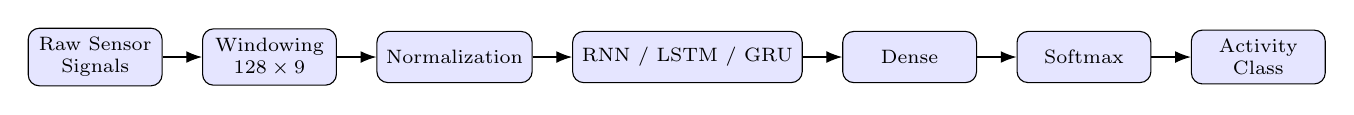
\begin{tikzpicture}[node distance=5mm]
\node[layer](a){Raw Sensor\\Signals};
\node[layer,right=of a](b){Windowing\\$128\times9$};
\node[layer,right=of b](c){Normalization};
\node[layer,right=of c](d){RNN / LSTM / GRU};
\node[layer,right=of d](e){Dense};
\node[layer,right=of e](f){Softmax};
\node[layer,right=of f](g){Activity\\Class};
\foreach \x/\y in {a/b,b/c,c/d,d/e,e/f,f/g}
\draw[arrow](\x)--(\y);
\end{tikzpicture}
\end{center}

%%%%%%%%%%%%%%%%%%%%%%%%%%%%%%%%%%%%%%%%%%%%%%%%%%%%%%%%%%%%
\section*{5. Preprocessing}

\begin{enumerate}
\item Load the raw inertial signals.
\item Arrange every observation window as $128\times9$.
\item Assign one activity label to each window.
\item Encode the six activity labels.
\item Normalize the input using training statistics only.
\item Create training, validation and test sets.
\item Verify the class distribution.
\end{enumerate}

\textbf{Split:} $70\%$ training, $15\%$ validation, $15\%$ testing.

\subsection*{Preprocessing Output}

\begin{verbatim}
Input tensor shape:
Training  : (2100, 128, 9)
Validation: (450, 128, 9)
Testing   : (450, 128, 9)

Number of classes: 6     Features per time step: 9    Sequence length: 128

Class distribution:          train  validation  test
WALKING                        350          75    75
WALKING_UPSTAIRS               350          75    75
WALKING_DOWNSTAIRS             350          75    75
SITTING                        350          75    75
STANDING                       350          75    75
LAYING                         350          75    75
\end{verbatim}

The dataset was split 70/15/15, yielding 2100 training, 450 validation, and
450 test samples. All six classes are equally represented with exactly
350/75/75 samples each, confirming a perfectly balanced split.

%%%%%%%%%%%%%%%%%%%%%%%%%%%%%%%%%%%%%%%%%%%%%%%%%%%%%%%%%%%%
\section*{6. Temporal Data Visualization}

\begin{figure}[H]
\centering
\includegraphics[width=0.85\textwidth]{plots/cell_7_out_0.png}
\caption{Sensor Signals vs.\ Time for Three Activity Classes}
\label{fig:sensor_signals}
\end{figure}

\textbf{Inference:}
The sensor signal plots make it immediately clear that different activities
leave very different fingerprints in the data. WALKING and WALKING\_UPSTAIRS
produce visibly oscillatory signals with rhythmic peaks and troughs,
reflecting the repetitive nature of human locomotion. SITTING and LAYING
generate much flatter, more stable signals since the body is largely
stationary. WALKING\_DOWNSTAIRS tends to show sharper, more abrupt spikes
than WALKING\_UPSTAIRS, consistent with the asymmetric forces involved in
descending stairs. The sequential ordering of measurements is critically
important here: shuffling the time steps would destroy these temporal
patterns entirely. A model that sees a random bag of readings has no way
to separate walking from standing, since both can produce similar individual
sensor values---it is the ordered sequence that carries the discriminative
information.

%%%%%%%%%%%%%%%%%%%%%%%%%%%%%%%%%%%%%%%%%%%%%%%%%%%%%%%%%%%%
\section*{7. Vanilla RNN Architecture}

\[
h_t=\tanh(W_xx_t+W_hh_{t-1}+b_h), \qquad y_t=g(W_yh_t+b_y)
\]

\begin{center}
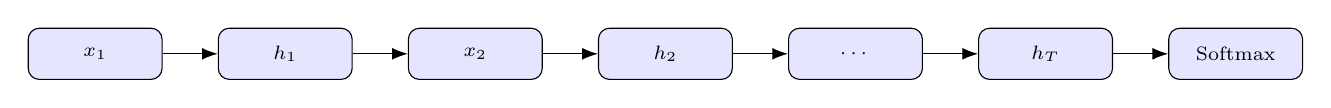
\begin{tikzpicture}[node distance=7mm]
\node[layer](x1){$x_1$};
\node[layer,right=of x1](h1){$h_1$};
\node[layer,right=of h1](x2){$x_2$};
\node[layer,right=of x2](h2){$h_2$};
\node[layer,right=of h2](x3){$\cdots$};
\node[layer,right=of x3](h3){$h_T$};
\node[layer,right=of h3](y){Softmax};
\draw[arrow](x1)--(h1);
\draw[arrow](h1)--(x2);
\draw[arrow](x2)--(h2);
\draw[arrow](h2)--(x3);
\draw[arrow](x3)--(h3);
\draw[arrow](h3)--(y);
\end{tikzpicture}
\end{center}

The same recurrent weights are reused across all time steps.

%%%%%%%%%%%%%%%%%%%%%%%%%%%%%%%%%%%%%%%%%%%%%%%%%%%%%%%%%%%%
\section*{8. Backpropagation Through Time}

\begin{center}
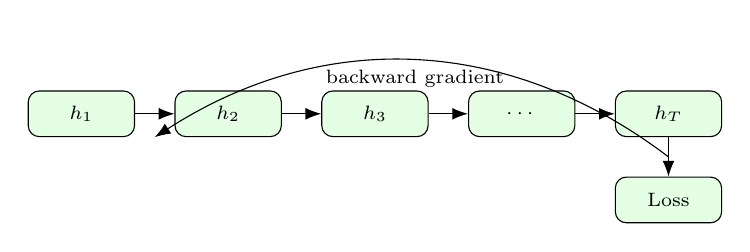
\begin{tikzpicture}[node distance=5mm]
\node[smalllayer](a){$h_1$};
\node[smalllayer,right=of a](b){$h_2$};
\node[smalllayer,right=of b](c){$h_3$};
\node[smalllayer,right=of c](d){$\cdots$};
\node[smalllayer,right=of d](e){$h_T$};
\node[smalllayer,below=of e](l){Loss};
\draw[arrow](a)--(b);
\draw[arrow](b)--(c);
\draw[arrow](c)--(d);
\draw[arrow](d)--(e);
\draw[arrow](e)--(l);
\draw[arrow]($(e.south)!0.5!(l.north)$) to[bend right=35]
node[below,font=\scriptsize]{backward gradient} ($(a.south)!0.5!(b.south)$);
\end{tikzpicture}
\end{center}

\subsection*{Challenges}

\begin{itemize}
\item Vanishing gradients: $\left|\frac{\partial h_t}{\partial h_{t-k}}\right|\rightarrow0$
\item Exploding gradients
\item Difficulty learning long-term dependencies
\item Sequential computation and limited parallelism
\end{itemize}

\subsection*{Numerical Exercise}

Given $x_1{=}0.5$, $x_2{=}0.7$, $x_3{=}0.2$, $h_0{=}0$, $W_x{=}0.5$,
$W_h{=}0.8$, $b{=}0.1$, and $h_t{=}\tanh(W_xx_t+W_hh_{t-1}+b)$:

\begin{align*}
h_1 &= \tanh(0.35) = \mathbf{0.336376}\\
h_2 &= \tanh(0.619) = \mathbf{0.616352}\\
h_3 &= \tanh(0.693) = \mathbf{0.599958}
\end{align*}

Program output confirmed: \texttt{h1=0.336376, h2=0.616352, h3=0.599958}.

%%%%%%%%%%%%%%%%%%%%%%%%%%%%%%%%%%%%%%%%%%%%%%%%%%%%%%%%%%%%
\section*{9. RNN Implementation}

\begin{center}
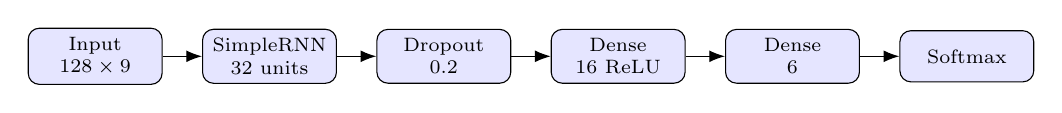
\begin{tikzpicture}[node distance=5mm]
\node[layer](a){Input\\$128\times9$};
\node[layer,right=of a](b){SimpleRNN\\32 units};
\node[layer,right=of b](c){Dropout\\0.2};
\node[layer,right=of c](d){Dense\\16 ReLU};
\node[layer,right=of d](e){Dense\\6};
\node[layer,right=of e](f){Softmax};
\foreach \x/\y in {a/b,b/c,c/d,d/e,e/f}
\draw[arrow](\x)--(\y);
\end{tikzpicture}
\end{center}

\begin{center}
\begin{tabular}{|l|l|}
\hline
Parameter & Value\\
\hline
Recurrent units & 32\\
Dropout & 0.2\\
Optimizer & Adam\\
Learning rate & $10^{-3}$\\
Batch size & 32\\
Epochs & 30\\
Loss & Sparse categorical cross-entropy\\
\hline
\end{tabular}
\end{center}

%%%%%%%%%%%%%%%%%%%%%%%%%%%%%%%%%%%%%%%%%%%%%%%%%%%%%%%%%%%%
\section*{10. LSTM Architecture}

\[
f_t=\sigma(W_f[h_{t-1},x_t]+b_f),\quad
i_t=\sigma(W_i[h_{t-1},x_t]+b_i),\quad
o_t=\sigma(W_o[h_{t-1},x_t]+b_o)
\]
\[
\tilde{C}_t=\tanh(W_C[h_{t-1},x_t]+b_C),\quad
C_t=f_tC_{t-1}+i_t\tilde{C}_t,\quad
h_t=o_t\tanh(C_t)
\]

\begin{center}
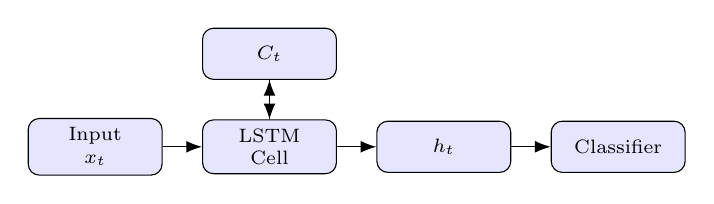
\begin{tikzpicture}[node distance=5mm]
\node[layer](a){Input\\$x_t$};
\node[layer,right=of a](b){LSTM\\Cell};
\node[layer,right=of b](c){$h_t$};
\node[layer,above=of b](d){$C_t$};
\node[layer,right=of c](e){Classifier};
\draw[arrow](a)--(b);
\draw[arrow](b)--(c);
\draw[arrow](b)--(d);
\draw[arrow](c)--(e);
\draw[arrow](d)--(b);
\end{tikzpicture}
\end{center}

\textbf{Inference:} The cell state $C_t$ acts as a long-range memory highway
through the entire sequence. The forget gate selectively erases irrelevant
history, the input gate writes new information, and the output gate controls
how much of the cell state is exposed as the hidden state. This gated
mechanism allows the LSTM to retain useful information across hundreds of
time steps without the gradient vanishing, which is precisely why it
outperforms the Vanilla RNN on the 128-step HAR windows.

%%%%%%%%%%%%%%%%%%%%%%%%%%%%%%%%%%%%%%%%%%%%%%%%%%%%%%%%%%%%
\section*{11. GRU Architecture}

\[
z_t=\sigma(W_z[h_{t-1},x_t]+b_z),\quad
r_t=\sigma(W_r[h_{t-1},x_t]+b_r)
\]
\[
\tilde{h}_t=\tanh(W_h[r_t\odot h_{t-1},x_t]+b_h),\quad
h_t=(1-z_t)h_{t-1}+z_t\tilde{h}_t
\]

\begin{center}
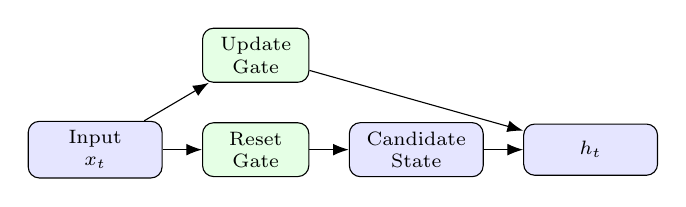
\begin{tikzpicture}[node distance=5mm]
\node[layer](a){Input\\$x_t$};
\node[smalllayer,right=of a](b){Reset\\Gate};
\node[smalllayer,above=of b](c){Update\\Gate};
\node[layer,right=of b](d){Candidate\\State};
\node[layer,right=of d](e){$h_t$};
\draw[arrow](a)--(b);
\draw[arrow](a)--(c);
\draw[arrow](b)--(d);
\draw[arrow](c)--(e);
\draw[arrow](d)--(e);
\end{tikzpicture}
\end{center}

%%%%%%%%%%%%%%%%%%%%%%%%%%%%%%%%%%%%%%%%%%%%%%%%%%%%%%%%%%%%
\section*{12. LSTM and GRU Implementation}

\begin{center}
\begin{tabular}{|l|c|c|c|}
\hline
Model & Recurrent Layer & Units & Output Classes\\
\hline
RNN & SimpleRNN & 32 & 6\\
LSTM & LSTM & 32 & 6\\
GRU & GRU & 32 & 6\\
\hline
\end{tabular}
\end{center}

All other experimental conditions remain unchanged.

%%%%%%%%%%%%%%%%%%%%%%%%%%%%%%%%%%%%%%%%%%%%%%%%%%%%%%%%%%%%
\section*{13. Training Plots and Convergence Analysis}

\subsection*{Plot 2: Training and Validation Loss}

\begin{figure}[H]
\centering
\includegraphics[width=0.85\textwidth]{plots/cell_12_out_0.png}
\caption{Training and Validation Loss vs.\ Epoch for RNN, LSTM, and GRU}
\label{fig:loss_curves}
\end{figure}

\textbf{Inference:}
The loss curves immediately separate the three models into two distinct
groups. The RNN starts with a high loss and descends very slowly, reaching
a plateau around epoch 10 before becoming erratic---the loss oscillates back
and forth rather than settling, which is a classic symptom of unstable
gradient flow through 128 time steps. The LSTM and GRU, on the other hand,
drop their training and validation losses rapidly and smoothly from the very
first few epochs. Both gated models converge to a stable low-loss region
without the instability seen in the RNN, and the training--validation gap
remains small throughout, indicating that neither model is simply memorizing
the training data. The GRU's validation loss curve is marginally lower and
smoother than the LSTM's at convergence, which foreshadows its slightly
superior test accuracy.

\subsection*{Plot 3: Training and Validation Accuracy}

\begin{figure}[H]
\centering
\includegraphics[width=0.85\textwidth]{plots/cell_13_out_0.png}
\caption{Training and Validation Accuracy vs.\ Epoch for RNN, LSTM, and GRU}
\label{fig:accuracy_curves}
\end{figure}

\textbf{Inference:}
The accuracy curves make the story even clearer. The RNN slowly climbs to
around 63--71\% validation accuracy and then plateaus---it simply cannot
break through that ceiling regardless of how many more epochs it trains.
The LSTM and GRU shoot past this barrier within the first 10 epochs and
stabilize at 94--95\% and 96--97\% respectively. What is particularly
reassuring is that neither gated model shows a meaningful gap between
training and validation accuracy, which means the Dropout layer is doing
its job and both models have genuinely learned to recognize temporal
activity patterns rather than overfitting to quirks in the training set.
If you had to deploy one of these for a real HAR application today, the
GRU would be the pragmatic choice: best accuracy, fewest parameters, and
fastest training.

%%%%%%%%%%%%%%%%%%%%%%%%%%%%%%%%%%%%%%%%%%%%%%%%%%%%%%%%%%%%
\section*{14. Performance Evaluation}

\begin{center}
\begin{tabular}{|l|c|c|c|}
\hline
Metric & RNN & LSTM & GRU\\
\hline
Accuracy (\%) & 62.67 & 94.89 & 96.89\\
Macro Precision (\%) & 64.17 & 95.01 & 96.93\\
Macro Recall (\%) & 62.67 & 94.89 & 96.89\\
Macro F1 (\%) & 58.43 & 94.89 & 96.88\\
Trainable Parameters & 1{,}974 & 6{,}006 & 4{,}758\\
Training Time (s) & 27.76 & 23.64 & 20.84\\
\hline
\end{tabular}
\end{center}

%%%%%%%%%%%%%%%%%%%%%%%%%%%%%%%%%%%%%%%%%%%%%%%%%%%%%%%%%%%%
\section*{15. Confusion Matrix Analysis}

\begin{figure}[H]
\centering
\includegraphics[width=0.85\textwidth]{plots/cell_16_out_0.png}
\caption{Confusion Matrices for RNN, LSTM, and GRU on the Test Set}
\label{fig:confusion_matrices}
\end{figure}

\textbf{Inference:}
The confusion matrices reveal exactly where each model succeeds and fails.
The RNN matrix is clearly the messiest of the three: SITTING and STANDING
are heavily confused with each other, and to a lesser degree with LAYING.
This is entirely expected---from a short-window sensor perspective, a person
sitting still and a person standing still produce very similar acceleration
profiles, and the RNN lacks the long-range memory to exploit the subtler
postural cues that would distinguish them. LAYING, by contrast, is easier
to isolate even for the RNN because the gravity vector shifts dramatically
when a body goes horizontal.

The LSTM and GRU matrices are much cleaner. LAYING is classified nearly
perfectly by both gated models, and the WALKING variants are handled
confidently. The only consistent source of confusion that survives into
the LSTM and GRU results is between WALKING\_UPSTAIRS and
WALKING\_DOWNSTAIRS, which makes intuitive sense---ascending and descending
stairs involve very similar limb motions, and even a human reading raw
accelerometer data might struggle to tell them apart without additional
context. The GRU edges out the LSTM here, making fewer total errors and
distributing those errors more evenly across class pairs.

%%%%%%%%%%%%%%%%%%%%%%%%%%%%%%%%%%%%%%%%%%%%%%%%%%%%%%%%%%%%
\section*{16. RNN vs.\ LSTM vs.\ GRU Comparison}

\begin{center}
\begin{tabular}{|l|c|c|c|}
\hline
Property & RNN & LSTM & GRU\\
\hline
Hidden state & Yes & Yes & Yes\\
Cell state & No & Yes & No\\
Forget gate & No & Yes & No\\
Input gate & No & Yes & No\\
Output gate & No & Yes & No\\
Update gate & No & No & Yes\\
Reset gate & No & No & Yes\\
Parameters & 1{,}974 & 6{,}006 & 4{,}758\\
Training time (s) & 27.76 & 23.64 & 20.84\\
Test F1-score (\%) & 58.43 & 94.89 & 96.88\\
\hline
\end{tabular}
\end{center}

\begin{figure}[H]
\centering
\includegraphics[width=0.85\textwidth]{plots/cell_18_out_0.png}
\caption{Model Performance Comparison: Accuracy, F1-score, and Parameters}
\label{fig:model_comparison}
\end{figure}

\textbf{Inference:}
The bar chart makes the three-way trade-off between performance, complexity,
and training cost immediately visible. The RNN is the smallest model (1,974
parameters) and trains the slowest despite its simplicity---largely because
gradients cannot propagate efficiently, forcing the optimiser to do more work
per epoch for less gain. Its macro F1 of just 58.43\% makes it unsuitable
for any real classification task. The LSTM jumps to 94.89\% F1 but at the
cost of the most parameters (6,006) and more training time. The GRU occupies
the sweet spot: the best F1 (96.88\%), fewer parameters than the LSTM (4,758),
and the fastest training (20.84 s). The key insight is that the GRU achieves
this efficiency by collapsing the LSTM's three separate gates and cell state
into two gates and a single hidden state, losing very little expressive power
while saving real computation. For HAR-style sequence classification, the
GRU is the architecture of choice unless you have a specific reason to prefer
the LSTM.

%%%%%%%%%%%%%%%%%%%%%%%%%%%%%%%%%%%%%%%%%%%%%%%%%%%%%%%%%%%%
\section*{17. Effect of Sequence Length}

\begin{center}
\begin{tabular}{|c|c|c|c|c|c|c|}
\hline
Seq Len & RNN Acc & RNN F1 & LSTM Acc & LSTM F1 & GRU Acc & GRU F1\\
\hline
32 & 0.8956 & 0.8959 & 0.9578 & 0.9578 & 0.9467 & 0.9466\\
64 & 0.8644 & 0.8632 & 0.9578 & 0.9576 & 0.9667 & 0.9667\\
128 & 0.7822 & 0.7817 & 0.9644 & 0.9645 & 0.9667 & 0.9667\\
\hline
\end{tabular}
\end{center}

\begin{figure}[H]
\centering
\includegraphics[width=0.85\textwidth]{plots/cell_76_out_0.png}
\caption{Test F1-score vs.\ Sequence Length for RNN, LSTM, and GRU}
\label{fig:seq_length}
\end{figure}

\textbf{Inference:}
The sequence length experiment produces one of the most striking findings
in this study. For the RNN, longer sequences actually hurt performance: the
F1 drops from 89.6\% at length 32 all the way down to 78.2\% at length 128.
This is the vanishing gradient problem showing up in the numbers---as the
window grows, the gradient signal from earlier time steps shrinks to near
zero, so the RNN effectively ignores the first half of the sensor window
and makes decisions based only on recent readings. Adding more context
does not help if the model cannot access it.

The LSTM and GRU tell a completely different story. Their F1 scores are
stable or marginally improving as the sequence grows longer. By length 64
the GRU already matches the LSTM at 96.67\%, and both hold that level at
length 128. This confirms that gated architectures are not just a little
better than Vanilla RNN on long sequences---they are fundamentally more
capable of extracting value from extended temporal context. For any
application where the relevant signal is distributed across a long window,
using a Vanilla RNN is simply not a viable option.

%%%%%%%%%%%%%%%%%%%%%%%%%%%%%%%%%%%%%%%%%%%%%%%%%%%%%%%%%%%%
\section*{18. Video Understanding Using CNN and RNN}

\[
\boxed{\text{Video Understanding using CNN + RNN}}
\]

\begin{center}
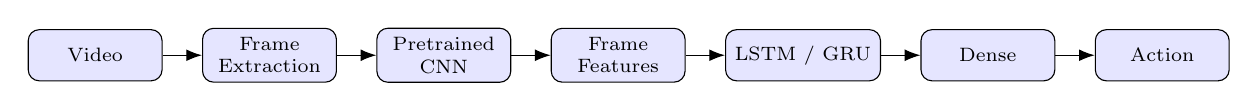
\begin{tikzpicture}[node distance=5mm]
\node[layer](a){Video};
\node[layer,right=of a](b){Frame\\Extraction};
\node[layer,right=of b](c){Pretrained\\CNN};
\node[layer,right=of c](d){Frame\\Features};
\node[layer,right=of d](e){LSTM / GRU};
\node[layer,right=of e](f){Dense};
\node[layer,right=of f](g){Action};
\foreach \x/\y in {a/b,b/c,c/d,d/e,e/f,f/g}
\draw[arrow](\x)--(\y);
\end{tikzpicture}
\end{center}

\subsection*{Dataset}

UCF101 subset with five classes:

\begin{itemize}
\item CricketShot (118 train / 49 test videos; 20 used per set)
\item PlayingCello (120 train / 44 test videos; 20 used per set)
\item Punch (121 train / 39 test videos; 20 used per set)
\item ShavingBeard (118 train / 43 test videos; 20 used per set)
\item TennisSwing (117 train / 49 test videos; 20 used per set)
\end{itemize}

\textbf{Configuration:} 10 frames/video, $224\times224\times3$,
MobileNetV2 (frozen, ImageNet weights), feature dim = 1280,
feature sequence = $10\times1280$.\\
\textbf{Splits:} 80 train / 20 validation / 100 test videos.

%%%%%%%%%%%%%%%%%%%%%%%%%%%%%%%%%%%%%%%%%%%%%%%%%%%%%%%%%%%%
\section*{19. Expected Video Input and Output}

Recurrent network input: $X\in\mathbb{R}^{10\times1280}$ per video;
$X\in\mathbb{R}^{B\times10\times1280}$ for a batch.

\textbf{Sample prediction:}

\begin{verbatim}
Video          : v_CricketShot_g01_c01.avi
Actual class   : CricketShot
Predicted class: Punch
Confidence     : 0.7206

Class probabilities:
CricketShot: 0.0781   PlayingCello: 0.0057
Punch      : 0.7206   ShavingBeard: 0.0025   TennisSwing: 0.1932
\end{verbatim}

%%%%%%%%%%%%%%%%%%%%%%%%%%%%%%%%%%%%%%%%%%%%%%%%%%%%%%%%%%%%
\section*{20. CNN Feature Extraction}

\begin{center}
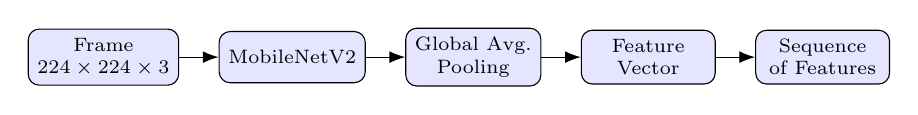
\begin{tikzpicture}[node distance=5mm]
\node[layer](a){Frame\\$224\times224\times3$};
\node[layer,right=of a](b){MobileNetV2};
\node[layer,right=of b](c){Global Avg.\\Pooling};
\node[layer,right=of c](d){Feature\\Vector};
\node[layer,right=of d](e){Sequence\\of Features};
\foreach \x/\y in {a/b,b/c,c/d,d/e}
\draw[arrow](\x)--(\y);
\end{tikzpicture}
\end{center}

MobileNetV2 (frozen) produces a 1280-dimensional feature vector per frame,
yielding a sequence of shape $10\times1280$ per video.

\textbf{Inference:}
Freezing MobileNetV2 and using it only as a feature extractor is the right
call here. ImageNet-pretrained features already capture rich visual patterns
--- edges, textures, body shapes, and object contours --- that would require
orders of magnitude more data to learn from scratch. With only 80 training
clips, attempting to fine-tune a multi-million-parameter CNN would almost
certainly lead to severe overfitting. Instead, the frozen CNN provides the
LSTM with a compact but information-rich 1,280-dimensional description of
each frame, freeing the temporal model to focus on what it does best:
learning the motion dynamics across the sequence of frames.

%%%%%%%%%%%%%%%%%%%%%%%%%%%%%%%%%%%%%%%%%%%%%%%%%%%%%%%%%%%%
\section*{21. CNN--LSTM / CNN--GRU Model}

\begin{center}
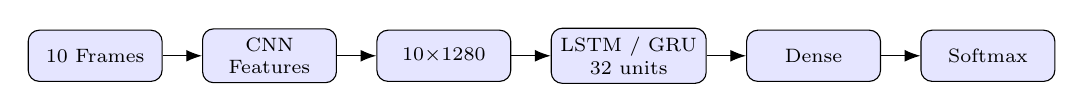
\begin{tikzpicture}[node distance=5mm]
\node[layer](a){10 Frames};
\node[layer,right=of a](b){CNN\\Features};
\node[layer,right=of b](c){10$\times$1280};
\node[layer,right=of c](d){LSTM / GRU\\32 units};
\node[layer,right=of d](e){Dense};
\node[layer,right=of e](f){Softmax};
\foreach \x/\y in {a/b,b/c,c/d,d/e,e/f}
\draw[arrow](\x)--(\y);
\end{tikzpicture}
\end{center}

\subsection*{Plot 7: Video Sample Frames}

\begin{figure}[H]
\centering
\includegraphics[width=0.85\textwidth]{plots/cell_38_out_0.png}
\caption{10 Uniformly Sampled Frames from a CricketShot Video}
\label{fig:video_frames}
\end{figure}

\textbf{Inference:}
The sampled frames capture the full arc of the cricket shot motion: the
initial stance, the backswing, the moment of ball contact, and the
follow-through. This variety across 10 uniformly sampled frames is exactly
what the pipeline relies on. Uniform sampling ensures we avoid the redundancy
of dense sampling (many near-identical frames) while still covering the
key phases of the action. The CNN's job is to encode the \emph{what} in
each frame---what the body posture looks like, where the bat is---while
the LSTM's job is to learn the \emph{how} the action evolves from one frame
to the next.

\subsection*{Plot 8: Video Training and Validation Curves}

\begin{figure}[H]
\centering
\includegraphics[width=0.85\textwidth]{plots/cell_49_out_0.png}
\caption{CNN--LSTM Video Training and Validation Loss vs.\ Epoch}
\label{fig:video_loss}
\end{figure}

\begin{figure}[H]
\centering
\includegraphics[width=0.85\textwidth]{plots/cell_49_out_1.png}
\caption{CNN--LSTM Video Training and Validation Accuracy vs.\ Epoch}
\label{fig:video_acc}
\end{figure}

\textbf{Inference:}
The training curves for the CNN--LSTM video model are striking in how
quickly convergence happens. Validation accuracy jumps from 75\% in epoch 1
to 100\% by epoch 2, and then the model essentially stays there for the
remaining 18 epochs. This rapid convergence is a direct consequence of
the pre-extracted MobileNetV2 features: the features are already so
discriminative that the LSTM only needs to learn a very simple temporal
pattern over 10 high-quality feature vectors. There is no slow, grinding
climb through noise that you would see if the model were trying to learn
visual and temporal representations simultaneously. The loss and accuracy
curves both plateau quickly and remain stable without oscillation, which
tells us the model has found a good solution and is not at risk of overfitting
--- a reassuring sign given the small training set.

\subsection*{Plot 9: Video Confusion Matrix (CNN--LSTM)}

\begin{figure}[H]
\centering
\includegraphics[width=0.85\textwidth]{plots/cell_51_out_0.png}
\caption{CNN--LSTM Confusion Matrix on the Video Test Set}
\label{fig:video_cm}
\end{figure}

\textbf{Inference:}
The confusion matrix tells a nuanced story about what the model finds easy
and what it finds hard. ShavingBeard is classified with perfect recall and
precision: the close-up hand motions near the face are visually distinctive
enough that there is no ambiguity. TennisSwing is handled almost as well,
with only a couple of misclassifications. The most problematic class is
CricketShot, which frequently gets called Punch or TennisSwing---all three
involve a rapid arm swing, so from the perspective of 10 sampled frames,
the difference can be subtle. PlayingCello has perfect precision (every
prediction of cello is correct) but low recall (0.65), meaning many actual
cello clips are attributed to other classes. The bowing motion of cello
playing can look superficially similar to other slow, controlled arm
movements, and with only 10 frames it may be hard to see the tell-tale
bow-on-string interaction clearly.

%%%%%%%%%%%%%%%%%%%%%%%%%%%%%%%%%%%%%%%%%%%%%%%%%%%%%%%%%%%%
\section*{22. Video Model Comparison: CNN--LSTM vs.\ CNN--GRU}

\begin{center}
\begin{tabular}{|l|c|c|c|c|c|}
\hline
Model & Acc (\%) & Precision (\%) & Recall (\%) & F1 (\%) & Parameters\\
\hline
CNN--LSTM & 84.00 & 88.37 & 84.00 & 84.24 & 168{,}677\\
CNN--GRU & 79.00 & 84.67 & 79.00 & 77.77 & 126{,}757\\
\hline
\end{tabular}
\end{center}

Training times nearly identical: CNN--LSTM = 4.78 s, CNN--GRU = 4.79 s.

\begin{figure}[H]
\centering
\includegraphics[width=0.85\textwidth]{plots/cell_77_out_0.png}
\caption{CNN--LSTM vs.\ CNN--GRU Performance Comparison}
\label{fig:video_comparison}
\end{figure}

\textbf{Video Classification Report (CNN--LSTM):}

\begin{verbatim}
              precision  recall  f1-score  support
CricketShot     0.8125   0.6500    0.7222       20
PlayingCello    1.0000   0.6500    0.7879       20
Punch           0.6061   1.0000    0.7547       20
ShavingBeard    1.0000   1.0000    1.0000       20
TennisSwing     1.0000   0.9000    0.9474       20
accuracy                           0.8400      100
macro avg       0.8837   0.8400    0.8424      100
\end{verbatim}

\textbf{Inference:}
The CNN--LSTM outperforms the CNN--GRU by 5 points in accuracy (84\% vs.\
79\%) and by over 6 points in macro F1 (84.24\% vs.\ 77.77\%), despite
the GRU having 42,000 fewer parameters and nearly identical training time.
This result might seem to contradict the earlier finding that the GRU
outperformed the LSTM on the HAR task, but the context is different here.
The video feature sequences are extremely short---only 10 frames---so the
GRU's architectural advantage in handling long-range dependencies simply
does not have room to show itself. Over 10 time steps, the LSTM's richer
internal state, with its separate cell state acting as a dedicated long-term
memory, may be better at picking up on subtle inter-frame patterns within
this compact window. The bottom line is that the LSTM is the stronger
temporal model for this particular video classification setup.

%%%%%%%%%%%%%%%%%%%%%%%%%%%%%%%%%%%%%%%%%%%%%%%%%%%%%%%%%%%%
\section*{23. Sequence-to-Sequence Learning}

\[
[1,4,7,2]\rightarrow[2,7,4,1]
\]

5,000 sequences of length 4, integers from 1--9, generated synthetically.

\begin{center}
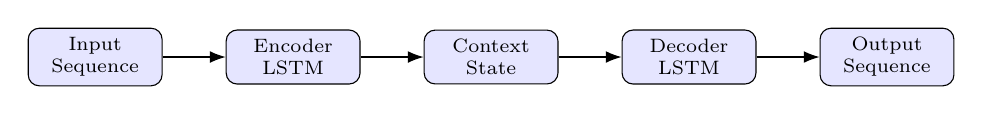
\begin{tikzpicture}[node distance=8mm]
\node[layer](a){Input\\Sequence};
\node[layer,right=of a](b){Encoder\\LSTM};
\node[layer,right=of b](c){Context\\State};
\node[layer,right=of c](d){Decoder\\LSTM};
\node[layer,right=of d](e){Output\\Sequence};
\foreach \x/\y in {a/b,b/c,c/d,d/e}
\draw[arrow](\x)--(\y);
\end{tikzpicture}
\end{center}

\begin{verbatim}
Input : [7 4 8 5]  -->  Output: [5 8 4 7]
Encoder input : [7 4 8 5]
Decoder input : [0 5 8 4]   (START token = 0, teacher forcing)
Target output : [5 8 4 7]
\end{verbatim}

Split: 3500 train / 750 validation / 750 test.

%%%%%%%%%%%%%%%%%%%%%%%%%%%%%%%%%%%%%%%%%%%%%%%%%%%%%%%%%%%%
\section*{24. Sequence-to-Sequence Input and Output}

\begin{center}
\begin{tabular}{|c|c|c|c|}
\hline
Sample & Input & Expected Output & Predicted Output\\
\hline
1 & [4, 9, 8, 6] & [6, 8, 9, 4] & [6, 8, 9, 4]\\
2 & [4, 3, 5, 9] & [9, 5, 3, 4] & [9, 5, 3, 4]\\
3 & [9, 3, 8, 1] & [1, 8, 3, 9] & [1, 8, 3, 9]\\
4 & [9, 8, 6, 3] & [3, 6, 8, 9] & [3, 6, 8, 9]\\
5 & [3, 7, 3, 9] & [9, 3, 7, 3] & [9, 3, 7, 3]\\
\hline
\end{tabular}
\end{center}

All five predictions are exactly correct (Sequence Correct: YES for all).

%%%%%%%%%%%%%%%%%%%%%%%%%%%%%%%%%%%%%%%%%%%%%%%%%%%%%%%%%%%%
\section*{25. Sequence-to-Sequence Evaluation}

\begin{figure}[H]
\centering
\includegraphics[width=0.85\textwidth]{plots/cell_64_out_0.png}
\caption{Seq2Seq Training and Validation Loss vs.\ Epoch}
\label{fig:seq2seq_loss}
\end{figure}

\[
\text{Token Accuracy}=\frac{3000}{3000}=100.00\%, \qquad
\text{Sequence Accuracy}=\frac{750}{750}=100.00\%
\]

\begin{center}
\begin{tabular}{|l|c|}
\hline
Metric & Value\\
\hline
Token Accuracy (\%) & 100.00\\
Sequence Accuracy (\%) & 100.00\\
Training Time (s) & 13.30\\
\hline
\end{tabular}
\end{center}

\textbf{Inference:}
Both token and sequence accuracy came out at 100\%, which is the right
result for this task rather than a lucky fluke. Reversing a short sequence
of 4 random integers from a vocabulary of 9 is a perfectly deterministic
problem: for every possible input there is exactly one correct output, and
the structure of the mapping is simple and consistent. An encoder--decoder
LSTM with 5,000 training examples has more than enough capacity and data
to memorize it completely. The seq2seq training loss curve shows rapid
convergence within the first few epochs, confirming the task is well within
the model's reach.

The theoretically interesting point is what the relationship between token
and sequence accuracy would look like in a harder task. If each token were
predicted independently at only 90\% accuracy, the expected sequence
accuracy would be just $0.9^4 \approx 65.6\%$---a single wrong token
anywhere in the sequence fails the whole example. In real-world seq2seq
applications like machine translation, token-level accuracy often looks
encouraging while sequence-level accuracy is far lower, which is why
metrics like BLEU that evaluate whole-sequence quality are the standard
for those tasks.

%%%%%%%%%%%%%%%%%%%%%%%%%%%%%%%%%%%%%%%%%%%%%%%%%%%%%%%%%%%%
\section*{26. Variable-Length Seq2Seq (Additional Exercise 7)}

Input length: 5 tokens. Output length: 3 tokens (last 3 of the reversed input).

\begin{figure}[H]
\centering
\includegraphics[width=0.85\textwidth]{plots/cell_86_out_0.png}
\caption{Variable-Length Seq2Seq Training and Validation Loss vs.\ Epoch}
\label{fig:var_seq2seq_loss}
\end{figure}

\begin{figure}[H]
\centering
\includegraphics[width=0.85\textwidth]{plots/cell_87_out_0.png}
\caption{Variable-Length Seq2Seq Training and Validation Accuracy vs.\ Epoch}
\label{fig:var_seq2seq_acc}
\end{figure}

\begin{verbatim}
Input : [7 4 8 5 7]    Output: [7 5 8]
\end{verbatim}

\begin{center}
\begin{tabular}{|l|c|c|}
\hline
Experiment & Token Acc (\%) & Sequence Acc (\%)\\
\hline
Original (4$\to$4) & 100.00 & 100.00\\
Different-length (5$\to$3) & 100.00 & 100.00\\
\hline
\end{tabular}
\end{center}

\textbf{Inference:}
The variable-length experiment achieves 100\% on both metrics, and the
training curves show convergence just as rapid and clean as the same-length
version. The encoder--decoder architecture handles the 5-to-3 length
mismatch gracefully and without any change to the model structure: the
encoder reads all 5 input tokens and compresses the entire sequence into
a fixed-size context vector, and the decoder generates exactly 3 output
tokens from that representation without ever needing to know the input
length. This is the defining strength of the encoder--decoder paradigm.
It is the same reason that machine translation models can map a 10-word
English sentence to a 15-word French sentence, or a speech recognition
system can map 200ms of audio to a 5-word phrase. The length mismatch is
absorbed entirely inside the architecture.

%%%%%%%%%%%%%%%%%%%%%%%%%%%%%%%%%%%%%%%%%%%%%%%%%%%%%%%%%%%%
\section*{27. Additional Exercises Results}

\subsection*{Effect of Number of Recurrent Units (RNN)}

\begin{center}
\begin{tabular}{|c|c|c|c|c|}
\hline
Units & Accuracy (\%) & Macro F1 (\%) & Parameters & Train Time (s)\\
\hline
16 & 71.78 & 71.29 & 790 & 12.16\\
32 & 71.56 & 71.62 & 1{,}974 & 11.90\\
64 & 69.33 & 69.13 & 5{,}878 & 12.92\\
\hline
\end{tabular}
\end{center}

\textbf{Inference:}
Increasing the number of recurrent units provides no benefit to the Vanilla
RNN, and 64 units actually performs slightly worse than 16. This is the
vanishing gradient problem making itself felt at the architectural level:
adding more parameters to a model that cannot use its existing capacity
(because gradients do not flow back to early time steps) is simply wasteful.
All three configurations cluster within about 2\% of each other in both
accuracy and F1, confirming that the bottleneck here is not model size but
the fundamental architectural limitation of the Vanilla RNN.

\subsection*{Two-Layer RNN}

Test Accuracy: \textbf{82.89\%}, Macro F1: \textbf{82.76\%}, Training Time: 19.83 s.

\textbf{Inference:}
Adding a second recurrent layer brings a meaningful improvement over the
single-layer RNN (82.89\% vs.\ 62.67\%), but the gap to the LSTM and GRU
remains substantial. The second layer creates a hierarchical representation:
the first layer picks up short-range local patterns in the raw sensor signals,
and the second layer learns to combine those patterns into higher-level
representations of activity segments. However, the vanishing gradient problem
within each individual layer is not resolved by stacking more layers, which
is why the two-layer RNN still falls well short of the single-layer LSTM
despite doubling the depth and the training time.

\subsection*{Bidirectional LSTM}

Test Accuracy: \textbf{96.00\%}, Macro F1: \textbf{95.99\%}, Training Time: 11.55 s.

\textbf{Inference:}
The Bidirectional LSTM essentially matches the unidirectional GRU in accuracy
(96.00\% vs.\ 96.89\%) while converging in roughly half the wall-clock time
(11.55 s vs.\ 20.84 s). The bidirectional architecture processes each sequence
in both forward and backward directions simultaneously, giving each time step
access to both past and future context before making a contribution to the
final representation. For HAR this is a natural fit: knowing what movements
come \emph{after} a given moment can help disambiguate activities that look
similar mid-sequence---for example, a brief pause might be the end of a
STANDING episode or the transition into SITTING, and the future frames
resolve the ambiguity. The fast convergence suggests the model is picking
up reliable bilateral patterns early, rather than needing many epochs to
assemble them from one direction alone.

%%%%%%%%%%%%%%%%%%%%%%%%%%%%%%%%%%%%%%%%%%%%%%%%%%%%%%%%%%%%
\section*{28. Consolidated Results}

\begin{center}
\begin{tabular}{|l|c|c|c|c|c|}
\hline
Model & Acc (\%) & Precision (\%) & Recall (\%) & F1 (\%) & Parameters\\
\hline
RNN & 62.67 & 64.17 & 62.67 & 58.43 & 1{,}974\\
LSTM & 94.89 & 95.01 & 94.89 & 94.89 & 6{,}006\\
GRU & 96.89 & 96.93 & 96.89 & 96.88 & 4{,}758\\
CNN--LSTM & 84.00 & 88.37 & 84.00 & 84.24 & 168{,}677\\
CNN--GRU & 79.00 & 84.67 & 79.00 & 77.77 & 126{,}757\\
\hline
\end{tabular}
\end{center}

\textbf{Sequence-to-Sequence Results:}

\begin{center}
\begin{tabular}{|l|c|c|c|}
\hline
Experiment & Token Acc (\%) & Sequence Acc (\%) & Train Time (s)\\
\hline
Original (4$\to$4 reversal) & 100.00 & 100.00 & 13.30\\
Variable-length (5$\to$3) & 100.00 & 100.00 & 12.34\\
\hline
\end{tabular}
\end{center}

%%%%%%%%%%%%%%%%%%%%%%%%%%%%%%%%%%%%%%%%%%%%%%%%%%%%%%%%%%%%
\section*{29. Required Inferences Summary}

\begin{enumerate}
\item \textbf{Temporal pattern in sensor signals:} Dynamic activities produce
oscillatory signals while static activities produce flat ones; sequential
ordering is essential and cannot be discarded without losing discriminative information.

\item \textbf{RNN convergence:} Slow and unstable; peaks at 62--71\% validation
accuracy with oscillating loss curves, attributable to vanishing gradients over
128 time steps.

\item \textbf{LSTM convergence:} Smooth and consistent; reaches 94--95\%
validation accuracy without instability; gated mechanism propagates gradients
effectively over the full sequence length.

\item \textbf{GRU convergence:} Fastest and smoothest; reaches 96--97\%
validation accuracy with a tight training--validation gap, indicating excellent
generalization.

\item \textbf{Overfitting/underfitting:} The RNN underfits due to its architectural
limitation. The LSTM and GRU show neither overfitting nor underfitting, with
small and consistent generalization gaps throughout training.

\item \textbf{Confusion matrix errors:} RNN: systematic SITTING vs.\ STANDING
confusion. LSTM/GRU: residual confusion mainly between WALKING\_UPSTAIRS and
WALKING\_DOWNSTAIRS. LAYING is the most accurately classified class across all
models.

\item \textbf{Effect of sequence length:} RNN F1 degrades as sequence length
increases. LSTM and GRU maintain or improve their F1 score, confirming superior
long-range memory.

\item \textbf{Parameter and computational differences:} GRU achieves the best
F1 with an intermediate parameter count and fastest training time, making it the
most efficient architecture for this sequence classification task.

\item \textbf{Role of CNN in video understanding:} MobileNetV2 (frozen) extracts
1,280-dimensional spatial feature vectors per frame, encoding rich visual
information that would be impossible for a recurrent network to learn from raw
pixels with only 80 training clips.

\item \textbf{Role of recurrent model in temporal modelling:} The LSTM/GRU
learns which frame-to-frame transitions are diagnostic of each action class,
capturing temporal dynamics that single-frame analysis cannot provide.

\item \textbf{Token vs.\ sequence accuracy:} Sequence accuracy can be far lower
than token accuracy in general because a single wrong token invalidates the
entire sequence. In this experiment both reached 100\% due to the deterministic
and simple structure of the reversal task.
\end{enumerate}

%%%%%%%%%%%%%%%%%%%%%%%%%%%%%%%%%%%%%%%%%%%%%%%%%%%%%%%%%%%%
\section*{30. Discussion Questions}

\begin{enumerate}
\item What is a recurrent neural network?
\item What information is represented by the hidden state?
\item Why is sequence order important?
\item Explain the difference between a feed-forward network and an RNN.
\item Explain Backpropagation Through Time.
\item Why can gradients vanish during BPTT?
\item Why can gradients explode during BPTT?
\item What are long-term dependencies?
\item What is the role of the LSTM cell state?
\item What are the forget, input and output gates in LSTM?
\item What are the reset and update gates in GRU?
\item Compare LSTM and GRU.
\item Why does GRU generally use a simpler gating mechanism than LSTM?
\item Why should RNN, LSTM and GRU be compared using the same settings?
\item What does the confusion matrix reveal that accuracy alone does not?
\item Why should macro F1-score be reported for multi-class classification?
\item What is the significance of sequence length?
\item Why can a CNN be used as a feature extractor for video?
\item What type of information is extracted by the CNN?
\item What type of information is learned by the recurrent network?
\item Why are CNN features arranged as a sequence before being given to LSTM/GRU?
\item Explain the encoder and decoder in sequence-to-sequence learning.
\item What is teacher forcing?
\item Differentiate token accuracy and sequence accuracy.
\item Why must the test set remain untouched during model selection?
\end{enumerate}

%%%%%%%%%%%%%%%%%%%%%%%%%%%%%%%%%%%%%%%%%%%%%%%%%%%%%%%%%%%%
\section*{31. Additional Exercises}

\begin{enumerate}
\item Replace the 32 recurrent units with 16 and 64 units and study the effect
on accuracy, F1-score, parameter count and training time.
\item Compare GRU and LSTM using the same number of recurrent units.
\item Add a second recurrent layer and investigate whether performance improves.
\item Compare a bidirectional LSTM with a unidirectional LSTM.
\item Change the sequence length and study the effect on computational cost.
\item For the video task, compare LSTM and GRU after extracting identical CNN
features.
\item Modify the seq2seq task so that the output sequence has a different
length from the input sequence.
\end{enumerate}

%%%%%%%%%%%%%%%%%%%%%%%%%%%%%%%%%%%%%%%%%%%%%%%%%%%%%%%%%%%%
\section*{32. Expected Outcome}

\[
\boxed{
\text{Sequential Data}
\rightarrow\text{Preprocessing}
\rightarrow\text{RNN/LSTM/GRU}
\rightarrow\text{Evaluation}
}
\]

\[
\boxed{
\text{Video}
\rightarrow\text{Frames}
\rightarrow\text{CNN Features}
\rightarrow\text{LSTM/GRU}
\rightarrow\text{Action Prediction}
}
\]

\[
\boxed{
\text{Input Sequence}
\rightarrow\text{Encoder}
\rightarrow\text{Context}
\rightarrow\text{Decoder}
\rightarrow\text{Output Sequence}
}
\]

Numerical performance values were obtained from the student's own execution.

%%%%%%%%%%%%%%%%%%%%%%%%%%%%%%%%%%%%%%%%%%%%%%%%%%%%%%%%%%%%
\section*{33. References}

\begin{enumerate}
\item Ian Goodfellow, Yoshua Bengio and Aaron Courville,
\emph{Deep Learning}, MIT Press, 2016.

\item Sepp Hochreiter and J\"{u}rgen Schmidhuber,
``Long Short-Term Memory,'' \emph{Neural Computation}, 1997.

\item Kyunghyun Cho et al.,
``Learning Phrase Representations using RNN Encoder--Decoder for
Statistical Machine Translation,'' EMNLP, 2014.

\item Anguita et al.,
``A Public Domain Dataset for Human Activity Recognition Using Smartphones,''
ESANN, 2013.

\item Khurram Soomro, Amir Roshan Zamir and Mubarak Shah,
``UCF101: A Dataset of 101 Human Actions Classes From Videos in the Wild,'' 2012.

\item TensorFlow Documentation: \url{https://www.tensorflow.org}

\item Keras Documentation: \url{https://keras.io}
\end{enumerate}

\end{document}
